\documentclass[11pt,a4paper]{article}
\usepackage[utf8]{inputenc}
\usepackage[T1]{fontenc}
\usepackage[spanish,es-noshorthands]{babel}
\usepackage{lmodern}
\usepackage{amsmath,amssymb,amsthm,mathtools}

\usepackage{graphicx}
\usepackage{booktabs}
\usepackage{tikz}
\usetikzlibrary{arrows.meta,positioning,calc}
\usepackage[margin=2.5cm]{geometry}
\usepackage[colorlinks=true,linkcolor=blue!50!black,citecolor=blue!50!black,urlcolor=blue!50!black]{hyperref}
\usepackage{xcolor}
\usepackage{caption}
\captionsetup{font=small,labelfont=bf}

\newtheorem{proposicion}{Proposición}
\theoremstyle{remark}
\newtheorem*{obs}{Observación}

\newcommand{\ket}[1]{\lvert #1\rangle}
\newcommand{\one}{\mathbf{1}}
\newcommand{\im}{\operatorname{Im}}
\newcommand{\re}{\operatorname{Re}}

\title{Caminata cuántica discreta con moneda arbitraria\\ y paredes reflectoras:\\ espectro exacto, simetrías y estadística de espaciamientos}
\author{Notas de trabajo}
\date{Octubre de 2026}

\begin{document}
\maketitle

\begin{abstract}
Estudiamos la caminata cuántica discreta en el tiempo sobre $n$ sitios con un
\emph{shift} condicional que rebota en las paredes y una moneda arbitraria de
$U(2)$. Mostramos que el \emph{shift} con rebote es equivalente a una traslación
en un anillo de $2n$ sitios y obtenemos el espectro exacto del operador de
evolución: $2(n-1)$ eigenfases de banda dadas por
$\cos\omega_m=|a|\cos(\pi m/n)$ y dos eigenvalores aislados, asociados a
estados de borde, que dependen sólo de $\im b$. Identificamos las simetrías del
operador (dos antiunitarias que emparejan niveles y una unitaria que existe
para una familia particular de monedas) y calculamos la distribución de
espaciamientos a primeros vecinos $P(s)$: sin \emph{unfolding} tiene forma
cerrada, no universal, y con el \emph{unfolding} exacto es un
\emph{picket fence} $P(s)=\delta(s-1)$. Todos los resultados se verificaron
numéricamente.
\end{abstract}

\noindent\fbox{\parbox{\dimexpr\linewidth-2\fboxsep-2\fboxrule}{\small
Estas notas se generaron en una conversación con Claude (Anthropic). La
conversación completa, con las derivaciones y el código, está en:\\
\url{https://claude.ai/code/session_01Nm9SnouRU3E6KaUBQ5eZvr}}}

\section{El modelo}

\paragraph{Espacio de Hilbert.}
$\mathcal H=\mathcal H_{\text{pos}}\otimes\mathcal H_{\text{moneda}}=\mathbb C^n\otimes\mathbb C^2$, con base
$\ket{j,s}$, $j=0,\dots,n-1$, $s\in\{R,L\}$. Si se quiere que las paredes estén en
$0$ y en $1$ basta tomar $x_j=j/(n-1)$.

\paragraph{Moneda.} Cualquier elemento de $U(2)$ se escribe como
\begin{equation}
C=e^{i\alpha}C_0,\qquad
C_0=\begin{pmatrix} a & b\\ -b^* & a^*\end{pmatrix},\qquad |a|^2+|b|^2=1,
\label{eq:moneda}
\end{equation}
y se aplica igual en todos los sitios: $\one_n\otimes C$. Escribimos
$a=|a|e^{i\varphi_a}$.

\paragraph{\emph{Shift} con rebote.} En el interior,
$S\ket{j,R}=\ket{j+1,R}$ ($j<n-1$) y $S\ket{j,L}=\ket{j-1,L}$ ($j>0$). En las
paredes la partícula se queda en su sitio y se invierte la quiralidad:
\begin{equation}
S\ket{n-1,R}=\ket{n-1,L},\qquad S\ket{0,L}=\ket{0,R}.
\end{equation}
Ésta es la forma natural del rebote, porque mantiene a $S$ unitario: la
alternativa $S\ket{n-1,R}=\ket{n-2,L}$ daría a $\ket{n-2,L}$ dos preimágenes.

\paragraph{Evolución.}
$\ket{\psi(t+1)}=U\ket{\psi(t)}$ con $U=S(\one_n\otimes C)$; si se quiere un
hamiltoniano efectivo, $U=e^{-iH_{\text{eff}}}$. Conviene quitar la fase global y
trabajar con $U_0=e^{-i\alpha}U$, cuyos eigenvalores escribimos como
$\mu=e^{i\theta}$.

\subsection{El rebote como condición periódica}

$S$ es una permutación de los $2n$ estados que forma un solo ciclo de longitud $2n$:
\begin{equation}
R_0\to R_1\to\cdots\to R_{n-1}\to L_{n-1}\to L_{n-2}\to\cdots\to L_0\to R_0 .
\end{equation}
Así, desplegado, el \emph{shift} con rebote es una traslación cíclica en un
\textbf{anillo de $2n$ sitios} (figura~\ref{fig:anillo}), con índice $m=j$ para
$R_j$ y $m=2n-1-j$ para $L_j$. La moneda rompe la invariancia traslacional del
anillo: acopla $R_j$ con $L_j$, es decir, los puntos $m$ y $2n-1-m$, que están
en posiciones especulares.

\begin{figure}[ht]
\centering
\begin{tikzpicture}[
  node distance=1.15cm,
  st/.style={circle,draw,minimum size=8mm,inner sep=0pt,font=\small},
  sh/.style={-{Stealth[length=2.2mm]},thick,blue!60!black},
  co/.style={dashed,orange!80!black,thick}]
  \foreach \j/\lab in {0/0,1/1,2/2,4/{n-1}} {
    \node[st] (R\j) at (1.6*\j,0) {$R_{\lab}$};
    \node[st] (L\j) at (1.6*\j,-1.6) {$L_{\lab}$};
    \draw[co] (R\j) -- (L\j);
  }
  \node at (1.6*3,0) {$\cdots$};
  \node at (1.6*3,-1.6) {$\cdots$};
  \draw[sh] (R0) -- (R1); \draw[sh] (R1) -- (R2);
  \draw[sh] (R2) -- ($(R2)+(0.9,0)$);
  \draw[sh] ($(R4)-(0.9,0)$) -- (R4);
  \draw[sh] (L1) -- (L0); \draw[sh] (L2) -- (L1);
  \draw[sh] ($(L2)+(0.9,0)$) -- (L2);
  \draw[sh] (L4) -- ($(L4)-(0.9,0)$);
  \draw[sh] (R4) to[out=0,in=0,looseness=1.6] node[right,font=\small]{pared} (L4);
  \draw[sh] (L0) to[out=180,in=180,looseness=1.6] node[left,font=\small]{pared} (R0);
  \node[font=\small,blue!60!black] at (9.3,-0.3) {$S$};
  \draw[sh] (8.7,-0.3) -- (9.05,-0.3);
  \node[font=\small,orange!80!black] at (9.3,-1.0) {$C$};
  \draw[co] (8.7,-1.0) -- (9.05,-1.0);
\end{tikzpicture}
\caption{El \emph{shift} con paredes reflectoras (flechas) es un solo ciclo de
longitud $2n$: un anillo. La moneda (líneas punteadas) acopla $R_j$ con $L_j$,
que en el anillo son puntos especulares.}
\label{fig:anillo}
\end{figure}

\section{Espectro exacto}

\begin{proposicion}\label{prop:espectro}
Para $a\neq0$ y $b\neq0$, los $2n$ eigenvalores de $U=S(\one_n\otimes C)$ son
\begin{align}
\lambda_{m,\pm}&=e^{i\alpha}e^{\pm i\omega_m},\qquad
\cos\omega_m=|a|\cos\frac{\pi m}{n},\qquad m=1,\dots,n-1, \label{eq:banda}\\
\lambda^{(\mathrm{ext})}_{\pm}&=e^{i\alpha}\Bigl(\pm\sqrt{1-(\im b)^2}+i\,\im b\Bigr). \label{eq:aislados}
\end{align}
\end{proposicion}

Las fases de banda dependen sólo de $|a|$: no dependen de $\varphi_a$ ni de la
fase de $b$. Los dos eigenvalores aislados dependen sólo de $\im b$; escritos
como fases son $e^{i\alpha}e^{i\vartheta}$ y $-e^{i\alpha}e^{-i\vartheta}$, con
$\sin\vartheta=\im b$.

\begin{proof}
\emph{1. Ecuaciones de eigenvalores.} Sean $\psi_j=(R_j,L_j)^T$,
$A=e^{i\alpha}a$, $B=e^{i\alpha}b$ y $(r_j,l_j)^T=C\psi_j$. La ecuación
$U\psi=\lambda\psi$ es
\begin{equation}
\lambda R_{j+1}=r_j\ (j\le n-2),\quad
\lambda L_{j-1}=l_j\ (j\ge1),\quad
\lambda R_0=l_0,\quad
\lambda L_{n-1}=r_{n-1}.
\end{equation}

\emph{2. Paredes como condiciones de frontera.} Agregamos dos sitios
ficticios, $R_n$ y $L_{-1}$. Con ellos las ecuaciones del bulto valen para todo
$j=0,\dots,n-1$, y las paredes se reducen a
\begin{equation}
R_0=L_{-1},\qquad R_n=L_{n-1}. \label{eq:cf}
\end{equation}

\emph{3. Ondas planas.} Con $(R_j,L_j)=z^j(u,v)$, el vector $(u,v)$ debe ser
eigenvector de la matriz $\operatorname{diag}(z^{-1},z)\,C$. Con $\lambda=e^{i\alpha}\mu$
esto da
\begin{equation}
a^*z^2-(\mu+\mu^{-1})z+a=0. \label{eq:cuadratica}
\end{equation}
Las raíces cumplen $z_1z_2=a/a^*$; escribiendo
$z_{1,2}=e^{i(\varphi_a\pm q)}$ se obtiene la relación de dispersión
$\cos\omega=|a|\cos q$ con $\mu=e^{i\omega}$. Para $b\neq0$ el eigenvector es
$(u,v)=(B,\ \lambda z-A)$.

\emph{4. Cuantización.} Tomamos $\psi=c_1(\cdot)_{z_1}+c_2(\cdot)_{z_2}$ y
definimos $f(z)=(B-\lambda)z+A$. Las condiciones~\eqref{eq:cf} quedan
\begin{equation}
\frac{c_1f(z_1)}{z_1}+\frac{c_2f(z_2)}{z_2}=0,\qquad
c_1z_1^{n-1}f(z_1)+c_2z_2^{n-1}f(z_2)=0,
\end{equation}
cuyo determinante se factoriza:
\begin{equation}
f(z_1)\,f(z_2)\,\frac{z_2^{\,n}-z_1^{\,n}}{z_1z_2}=0. \label{eq:det}
\end{equation}

\emph{5. Primera rama: la banda.} Si $z_1^n=z_2^n$, entonces $e^{2iqn}=1$ y
$q=\pi m/n$. Hay que excluir $q=0,\pi$, porque ahí $z_1=z_2$ y la solución es
trivial. Quedan $m=1,\dots,n-1$, y cada uno da dos fases $\pm\omega_m$: son
$2(n-1)$ estados extendidos.

\emph{6. Segunda rama: eigenvalores aislados.} Si $f(z)=0$ basta una sola
exponencial, y en toda la cadena $L_j=R_{j+1}$. Combinando $\lambda z=A+Bz$
con $\lambda=-e^{i\alpha}b^*+e^{i\alpha}a^*z$:
\begin{gather}
a^*z^2-2\re(b)\,z-a=0
\;\Longrightarrow\;
z_\pm=\frac{\re b\pm\sqrt{(\re b)^2+|a|^2}}{a^*},\\
\lambda_\pm=e^{i\alpha}\Bigl(i\,\im b\pm\sqrt{(\re b)^2+|a|^2}\Bigr),
\end{gather}
que es~\eqref{eq:aislados} porque $(\re b)^2+|a|^2=1-(\im b)^2$. En total hay
$2(n-1)+2=2n$ eigenvalores.
\end{proof}

\begin{obs}[Estados de borde]
Como $|z_+z_-|=1$, en general $|z_\pm|\neq1$: los dos estados aislados decaen
exponencialmente desde paredes opuestas, como $|z|^j$. Si $\re b=0$, entonces
$|z_\pm|=1$ y se vuelven extendidos.
\end{obs}

\paragraph{Casos de control.}
\begin{itemize}
\item \emph{Sin mezcla, $b=0$.} El espectro es
$\{e^{i\alpha}e^{i\pi m/n}\}_{m=0}^{2n-1}$: las raíces $2n$-ésimas de la unidad
por la fase global, exactamente el anillo de $2n$ sitios.
\item \emph{Hadamard, $a=b=1/\sqrt2$, $\alpha=0$.} La banda es
$\cos\omega_m=\cos(\pi m/n)/\sqrt2$ y los eigenvalores aislados son $\pm1$.
Como $\re b\neq0$ son estados de borde, con $|z_\pm|=|1\pm\sqrt2|$, localizados
uno en cada pared.
\end{itemize}

\paragraph{Verificación numérica.} Comparamos~\eqref{eq:banda}--\eqref{eq:aislados}
con la diagonalización directa de $U$ para $n=2,3,5,8,13$ y monedas
aleatorias de $U(2)$. El error máximo en las fases es $\sim10^{-15}$.

\begin{figure}[ht]
\centering
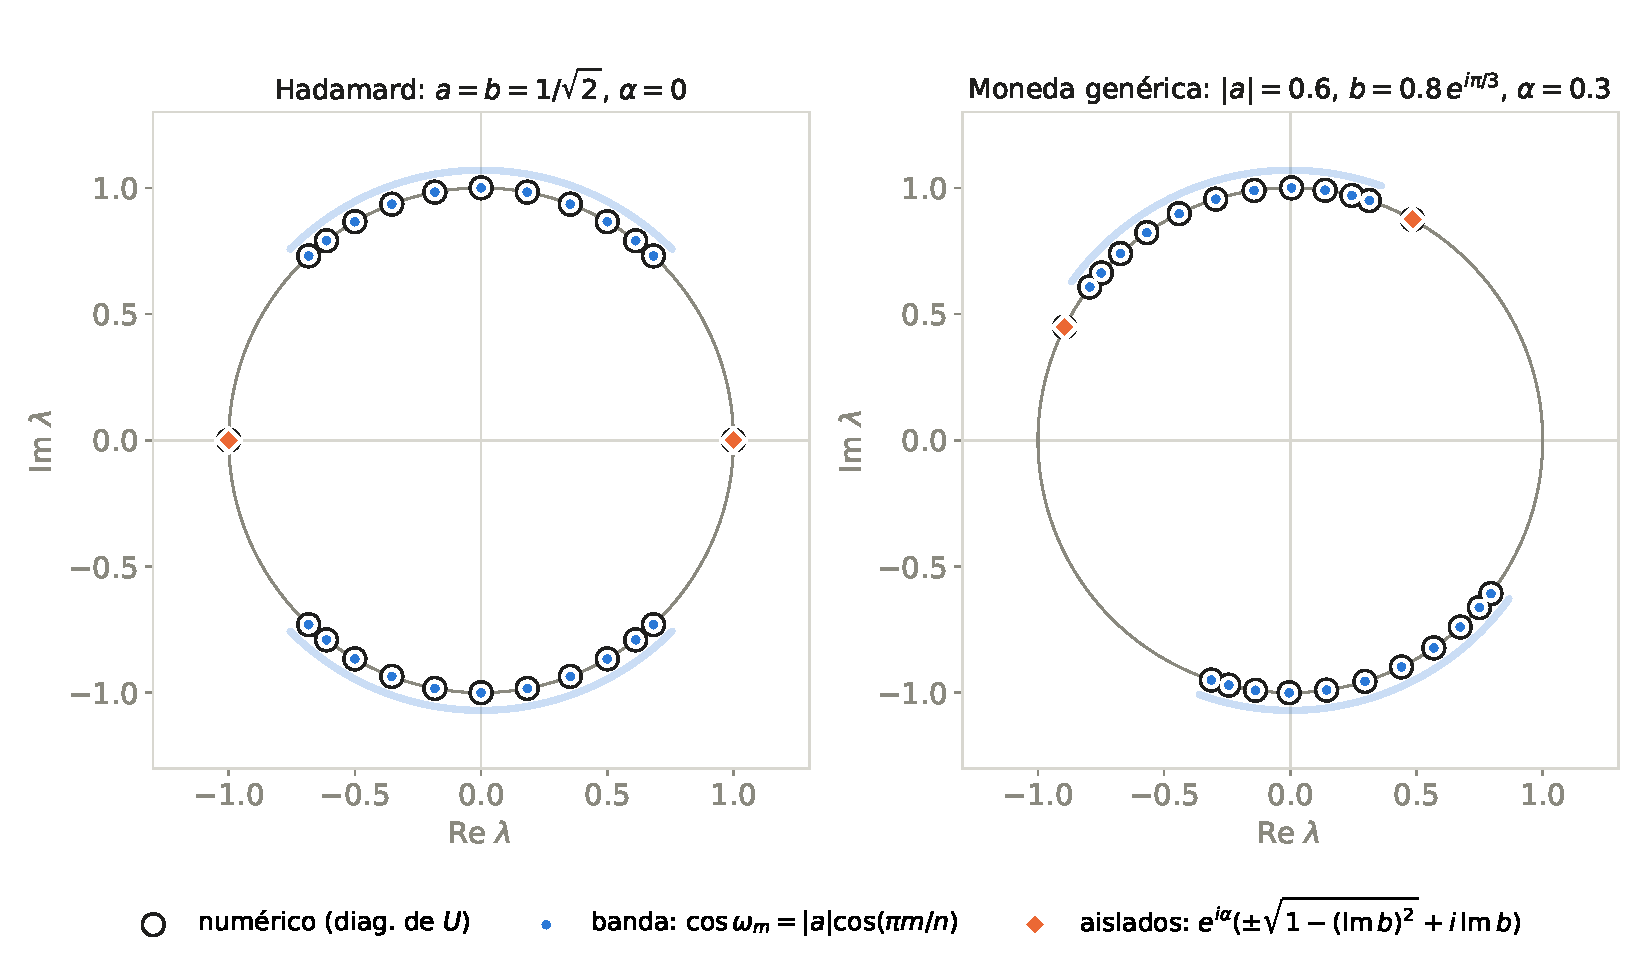
\includegraphics[width=\linewidth]{figs/eigenvalores.pdf}
\caption{Eigenvalores de $U$ en el círculo unitario para $n=12$. Los anillos
negros son la diagonalización numérica; los puntos azules, la
banda~\eqref{eq:banda}; los rombos naranjas, los eigenvalores
aislados~\eqref{eq:aislados}. Los arcos azul claro marcan la banda en el límite
$n\to\infty$, $\omega\in[\arccos|a|,\,\pi-\arccos|a|]$ y su reflejo, rotada por
$e^{i\alpha}$. Izquierda: Hadamard. Derecha: moneda genérica con $|a|=0.6$,
$b=0.8\,e^{i\pi/3}$, $\alpha=0.3$. Los eigenvalores aislados siempre caen en los
huecos espectrales.}
\label{fig:eigen}
\end{figure}

\section{Simetrías}

Usamos tres operadores:
\begin{itemize}
\item $P:\ \ket{j,R}\mapsto\ket{n-1-j,L}$, $\ket{j,L}\mapsto\ket{n-1-j,R}$: la
reflexión espacial con cambio de quiralidad. En el anillo es una traslación por
$n$, así que $PSP=S$; además $P(\one\otimes M)P=\one\otimes\sigma_xM\sigma_x$.
\item $\Gamma=(-1)^j\otimes\sigma_z$. Cumple $\Gamma S\Gamma=-S$, también en las
paredes, porque ahí $j$ no cambia pero la quiralidad sí.
\item $K$, la conjugación compleja en la base $\ket{j,s}$.
\end{itemize}

\begin{proposicion}\label{prop:sim}
Para cualquier moneda, el operador antiunitario $\Theta=P\Gamma K$ cumple
\begin{equation}
\Theta\,U_0\,\Theta^{-1}=-U_0,
\end{equation}
de modo que el espectro es invariante bajo $\mu\mapsto-\mu^*$, es decir,
$\theta\mapsto\pi-\theta$.
\end{proposicion}
\begin{proof}
$P\Gamma\,U_0^*\,\Gamma P=-S\bigl(\one\otimes\sigma_x\sigma_zC_0^*\sigma_z\sigma_x\bigr)
=-S\bigl(\one\otimes\sigma_yC_0^*\sigma_y\bigr)=-S(\one\otimes C_0)=-U_0$, usando
que $\sigma_yM^*\sigma_y=M$ para $M\in SU(2)$.
\end{proof}

Las otras dos simetrías existen sólo para algunas monedas:
\begin{itemize}
\item \emph{$\theta\mapsto-\theta$.} Conjugar cambia $(a,b)\mapsto(a^*,b^*)$ y, por
la proposición~\ref{prop:espectro}, el espectro sólo cambia a través de
$\im b\mapsto-\im b$. Por eso la banda siempre es simétrica bajo
$\theta\mapsto-\theta$, pero el espectro completo lo es sólo si $\im b=0$. Para
Hadamard, $U$ es real y la simetría es literalmente $KU_0K=U_0$.
\item \emph{Paridad $P$.} $PU_0P=S(\one\otimes\sigma_xC_0\sigma_x)$ con
$\sigma_xC_0\sigma_x=\bigl(\begin{smallmatrix}a^*&-b^*\\ b&a\end{smallmatrix}\bigr)$,
así que $[P,U_0]=0$ si y sólo si $a\in\mathbb R$ y $b\in i\mathbb R$.
\end{itemize}

\begin{table}[ht]
\centering\small
\begin{tabular}{@{}lll@{}}
\toprule
Simetría & Acción en el espectro & ¿Cuándo existe? \\
\midrule
$\Theta U_0\Theta^{-1}=-U_0$ (antiunitaria) & $\theta\to\pi-\theta$ & siempre \\
conjugación (antiunitaria) & $\theta\to-\theta$ & bulto: siempre; completo: si $\im b=0$ \\
$[P,U_0]=0$ (unitaria) & sectores $P=\pm1$ & si $a\in\mathbb R$, $b\in i\mathbb R$ \\
\bottomrule
\end{tabular}
\caption{Simetrías de $U_0=e^{-i\alpha}U$. Las tres se verificaron
numéricamente para Hadamard, para una moneda genérica y para $a=0.6$, $b=0.8i$.}
\label{tab:sim}
\end{table}

\paragraph{Consecuencias para la estadística.}
Las dos simetrías antiunitarias no dividen el espacio en sectores
independientes: \emph{emparejan} niveles. Para la estadística hay que quedarse
con el dominio fundamental $0<\theta\le\pi/2$, que contiene unos $n/2$ niveles
independientes; con el espectro completo cada espaciamiento aparece repetido.

Cuando existe $P$, los dos sectores se \emph{intercalan perfectamente}:
ordenando los niveles por fase, la paridad alterna entre $+1$ y $-1$ (lo
verificamos para $n=7$). Por eso, a diferencia de un sistema caótico,
superponer los sectores aquí no produce estadística de Poisson, y cada sector
por separado también es un \emph{picket fence}.

\section{Distribución de espaciamientos a primeros vecinos}

\subsection{Sin \emph{unfolding}}
Los espaciamientos dentro de la banda son
$\Delta\theta_m\simeq\frac{\pi}{n}\,g(q)$, con
\begin{equation}
g(q)=\frac{d\omega}{dq}=\frac{|a|\sin q}{\sqrt{1-|a|^2\cos^2q}},
\end{equation}
y $q=\pi m/n$ distribuido uniformemente en $(0,\pi)$ cuando $n\to\infty$.
Cambiando de variable a $x=\sin q$, en unidades de $\pi/n$:
\begin{equation}
P(s)=\frac{2}{\pi}\,\frac{|b|/|a|}{(1-s^2)\sqrt{1-s^2/|a|^2}},\qquad 0\le s<|a|.
\label{eq:Ps}
\end{equation}
Está normalizada: con $s=|a|\sin t$,
$\int_0^{|a|}P\,ds=\frac{2|b|}{\pi}\int_0^{\pi/2}\frac{dt}{1-|a|^2\sin^2t}=1$.
La media dentro de la banda es $\kappa=2\arcsin|a|/\pi$; en la
figura~\ref{fig:nns} se grafica $\tilde P(\tilde s)=\kappa P(\kappa\tilde s)$
con $\tilde s=s/\kappa$.

La distribución~\eqref{eq:Ps} cumple $P(0)\neq0$, así que no hay repulsión de
niveles, y diverge como $(|a|-s)^{-1/2}$ en el centro de la banda: es una
singularidad de van Hove. Su forma refleja sólo la densidad de estados y no
tiene nada de universal.

\subsection{Con \emph{unfolding}}
La función de conteo exacta,
\begin{equation}
N(\theta)=\frac{n}{\pi}\arccos\!\Bigl(\frac{\cos\theta}{|a|}\Bigr),
\end{equation}
manda cada nivel a $x_m=m$. Todos los espaciamientos valen entonces~1 y
\begin{equation}
P(s)=\delta(s-1)
\end{equation}
para cualquier $n$; numéricamente, la desviación estándar es $\sim10^{-11}$.
Es el espectro más rígido posible: $\Sigma^2(L)$ y $\Delta_3(L)$ quedan acotados
en lugar de crecer como $L$ (Poisson) o como $\log L$ (Wigner--Dyson).

Si en cambio el \emph{unfolding} se hace ``a ciegas'', con un polinomio de grado
9 ajustado a la escalera, como se haría con datos reales, aparece un pico
angosto en $s\approx1$ más una cola. La cola viene de los bordes de la banda,
donde el polinomio no puede reproducir la singularidad de raíz cuadrada de
$N(\theta)$: es un artefacto, no física.

\begin{figure}[ht]
\centering
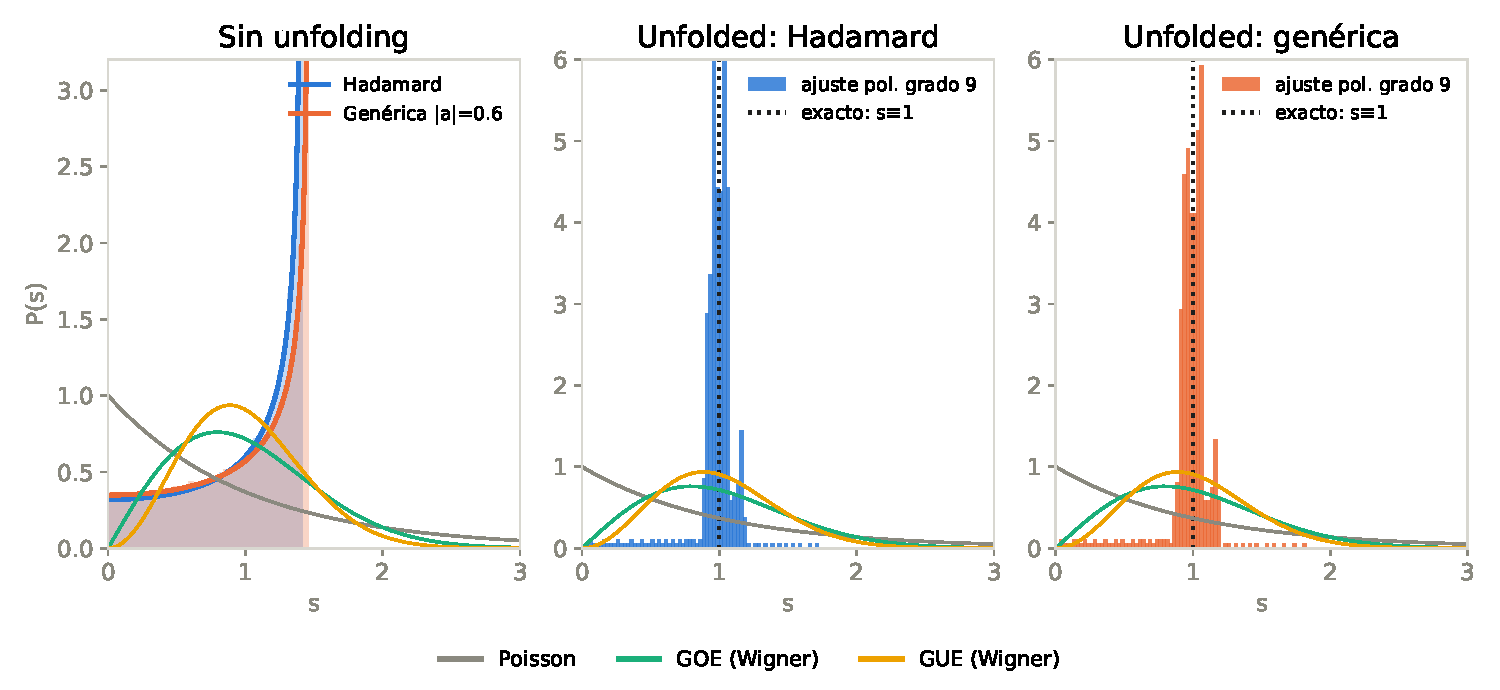
\includegraphics[width=\linewidth]{figs/nns.pdf}
\caption{$P(s)$ en el dominio fundamental $0<\theta\le\pi/2$, con
$\theta=\arg\lambda-\alpha$ y $n=1500$. Izquierda: sin \emph{unfolding}
(espaciamientos divididos entre la media en la banda); los histogramas son
numéricos y las curvas, la fórmula~\eqref{eq:Ps}. Centro y derecha: con
\emph{unfolding}; la línea punteada es el \emph{unfolding} exacto
($s\equiv1$) y el histograma, el ajuste polinomial. En los tres paneles se
muestran como referencia Poisson y las conjeturas de Wigner para GOE y GUE.}
\label{fig:nns}
\end{figure}

\section{Perspectivas}
El modelo es integrable: el número cuántico $m$ etiqueta todo el espectro de
banda. Para llegar a estadística de Wigner--Dyson hay que romper la
integrabilidad, por ejemplo con monedas que dependan del sitio. Con monedas
aleatorias, en una dimensión se espera localización de Anderson y $P(s)$ de
Poisson. Con monedas deterministas pero dependientes de $j$, la tabla de
simetrías~\ref{tab:sim} se vuelve la pregunta central: según qué
antiunitarias sobrevivan, el ensamble esperado sería COE o CUE, y habría que
desimetrizar respecto de las que emparejan niveles.

\appendix
\section{Código}
Los scripts en Python que acompañan estas notas son:
\begin{itemize}
\item \texttt{qw.py}: construye $U$ y compara el espectro numérico con la
proposición~\ref{prop:espectro}.
\item \texttt{sym.py}: verifica las relaciones de la tabla~\ref{tab:sim} y la
alternancia de paridad.
\item \texttt{plot\_tex.py}, \texttt{ps\_tex.py}: generan las
figuras~\ref{fig:eigen} y~\ref{fig:nns}.
\end{itemize}

\end{document}
